\documentclass[aspectratio=169,10pt,fontset=none]{ctexbeamer}

\usepackage{amsmath,amssymb,mathtools}
\usepackage{booktabs,tabularx,array}
\usepackage{graphicx}
\usepackage{tikz}
\usetikzlibrary{arrows.meta,positioning,shapes.geometric}
\usepackage{listings}
\usepackage{xcolor}

\setCJKmainfont{Noto Serif CJK SC}
\setCJKsansfont{Noto Sans CJK SC}
\setCJKmonofont{Noto Sans Mono CJK SC}
\setsansfont{Avenir Next}
\setmonofont{Menlo}

\usetheme{Madrid}
\usecolortheme{default}
\definecolor{CourseNavy}{HTML}{17365D}
\definecolor{CourseTeal}{HTML}{168C8C}
\definecolor{CourseOrange}{HTML}{D97706}
\definecolor{CourseLight}{HTML}{EEF4F8}
\definecolor{CourseRed}{HTML}{B42318}
\setbeamercolor{structure}{fg=CourseNavy}
\setbeamercolor{palette primary}{bg=CourseNavy,fg=white}
\setbeamercolor{palette secondary}{bg=CourseTeal,fg=white}
\setbeamercolor{palette tertiary}{bg=CourseNavy!85,fg=white}
\setbeamercolor{frametitle}{bg=CourseNavy,fg=white}
\setbeamercolor{block title}{bg=CourseNavy!12,fg=CourseNavy}
\setbeamercolor{block body}{bg=CourseLight!70,fg=black}
\setbeamercolor{alerted text}{fg=CourseRed}
\setbeamertemplate{navigation symbols}{}
\setbeamertemplate{caption}[numbered]
\setbeamertemplate{itemize item}{\color{CourseTeal}$\blacktriangleright$}
\setbeamertemplate{itemize subitem}{\color{CourseOrange}$\bullet$}
\setbeamertemplate{section in toc}[sections numbered]
\setbeamertemplate{subsection in toc}[square]

\newcommand{\E}{\mathbb{E}}
\newcommand{\Var}{\operatorname{Var}}
\newcommand{\Cov}{\operatorname{Cov}}
\newcommand{\dd}{\,\mathrm{d}}
\newcommand{\Normal}{\mathcal{N}}
\newcommand{\code}[1]{\texttt{#1}}
\newcommand{\good}[1]{\textcolor{CourseTeal}{#1}}
\newcommand{\warn}[1]{\textcolor{CourseOrange}{#1}}

\lstset{
  language=Python,
  basicstyle=\ttfamily\scriptsize,
  keywordstyle=\color{CourseNavy}\bfseries,
  commentstyle=\color{CourseTeal!80!black},
  stringstyle=\color{CourseOrange!90!black},
  showstringspaces=false,
  frame=single,
  rulecolor=\color{CourseNavy!25},
  backgroundcolor=\color{CourseLight!55},
  columns=fullflexible,
  keepspaces=true
}

\title[金融 SDE 的数值模拟]{金融随机微分方程的数值模拟}
\subtitle{从欧拉法到嵌套网格验证：PDE 数值解课程项目汇报}
\author[课程项目汇报]{姓名：\underline{\hspace{3cm}}\qquad 学号：\underline{\hspace{3cm}}}
\institute{数值偏微分方程课程}
\date{2026 年 9 月}

\AtBeginSection[]{
  \begin{frame}[plain]
    \vfill
    \centering
    {\usebeamerfont{title}\color{CourseNavy}\insertsectionnumber.\ \insertsectionhead\par}
    \vspace{0.8em}
    {\color{CourseTeal}\rule{0.56\linewidth}{1.2pt}}
    \vfill
  \end{frame}
}

\begin{document}

\begin{frame}
  \titlepage
\end{frame}

\begin{frame}{这份汇报希望解决什么问题？}
  \begin{block}{面向的听众}
    只学过常微分方程欧拉法和基础概率论；不要求随机微积分或金融知识。
  \end{block}
  \begin{enumerate}
    \item 如何把随机微分方程放到时间网格上计算？
    \item Monte Carlo 为什么能估计期望？误差条怎样得到？
    \item Euler--Maruyama 与 Milstein 的差别在哪里？
    \item ``强收敛''与``弱收敛''分别回答什么问题？
    \item 没有解析解时，怎样用嵌套网格构造可信的数值参考？
    \item 如何读懂本项目的图、表和最终结论？
  \end{enumerate}
\end{frame}

\begin{frame}{整项工作的主线}
  \centering
  \begin{tikzpicture}[
    node distance=7mm and 7mm,
    box/.style={draw=CourseNavy,rounded corners,fill=CourseLight,
      minimum width=2.65cm,minimum height=1.0cm,align=center,font=\small},
    arr/.style={-{Latex[length=2.5mm]},thick,draw=CourseTeal}
  ]
    \node[box] (model) {连续随机模型\\$\dd Z=a(Z)\dd t+b(Z)\dd W$};
    \node[box,right=of model] (grid) {时间网格\\$t_n=nh$};
    \node[box,right=of grid] (scheme) {离散格式\\EM / Milstein};
    \node[box,right=of scheme] (mc) {重复抽样\\Monte Carlo};
    \node[box,below=12mm of grid] (error) {误差与置信区间\\强 / 弱收敛};
    \node[box,right=of error] (evidence) {实验图表\\斜率、误差条、诊断};
    \draw[arr] (model)--(grid);
    \draw[arr] (grid)--(scheme);
    \draw[arr] (scheme)--(mc);
    \draw[arr] (mc)|-(evidence);
    \draw[arr] (scheme)--(error);
    \draw[arr] (error)--(evidence);
  \end{tikzpicture}
  \vspace{1em}

  \begin{alertblock}{数值分析的核心}
    不是只运行一次程序，而是说明：离散格式是什么、误差怎样缩小、统计噪声有多大、结论能否复现。
  \end{alertblock}
\end{frame}

\begin{frame}{它与数值 PDE 课程有什么关系？}
  对一维扩散过程
  \[
    \dd S_t=a(S_t)\dd t+b(S_t)\dd W_t,
  \]
  定义条件期望
  \[
    u(t,s)=\E\!\left[\varphi(S_T)\mid S_t=s\right].
  \]
  在适当条件下，$u$ 满足后向 Kolmogorov 方程
  \[
    u_t+a(s)u_s+\frac12 b(s)^2u_{ss}=0,
    \qquad u(T,s)=\varphi(s).
  \]
  \begin{block}{两条求解路线}
    \begin{itemize}
      \item PDE 路线：在 $(t,s)$ 网格上离散偏导数；
      \item 本项目路线：在时间上离散随机轨道，再用 Monte Carlo 求平均。
    \end{itemize}
  \end{block}
  本项目不要求实现 PDE 求解器，但仍在研究\alert{离散、收敛、稳定计算和误差量化}。
\end{frame}

\begin{frame}{报告中的两个模型与各自任务}
  \begin{tabularx}{\textwidth}{>{\bfseries}p{2.4cm}XX}
    \toprule
      & 模型一：GBM 基准 & 模型二：非仿射耦合模型 \\
    \midrule
    作用 & 有解析解，可检查程序和理论阶 & 更接近无解析解的真实数值任务 \\
    方法 & 精确采样、EM、Milstein & 对数变量上的 EM \\
    主要指标 & 强误差、弱误差、分布矩 & 嵌套参考、强差、非线性弱量 \\
    参考答案 & 同一布朗路径上的解析终值 & 更细网格上的数值解 \\
    关键困难 & 分清路径误差与期望误差 & 参考解本身也有离散误差 \\
    \bottomrule
  \end{tabularx}
  \vspace{0.7em}
  \centering
  \good{先用可验证模型建立信任，再把方法迁移到不能精确求解的模型。}
\end{frame}

\begin{frame}{汇报结构}
  \tableofcontents[hideallsubsections]
\end{frame}

\section{从欧拉法到随机时间步进}

\begin{frame}{回顾：常微分方程的显式欧拉法}
  对 ODE
  \[
    \frac{\dd y}{\dd t}=f(y),\qquad y(0)=y_0,
  \]
  建立均匀网格
  \[
    0=t_0<t_1<\cdots<t_N=T,\qquad h=\frac{T}{N}.
  \]
  在一个小区间上假设斜率近似不变：
  \[
    y(t_{n+1})-y(t_n)\approx f(y_n)h,
    \qquad \boxed{y_{n+1}=y_n+f(y_n)h}.
  \]
  \begin{block}{理解重点}
    连续变化被替换为许多小步；$h$ 越小，局部近似通常越好，但计算量增加。
  \end{block}
\end{frame}

\begin{frame}{随机微分方程只多了一种“随机步长”}
  一般 SDE 写成
  \[
    \boxed{\dd Z_t=a(Z_t)\dd t+b(Z_t)\dd W_t}.
  \]
  \begin{itemize}
    \item $a(Z_t)\dd t$：漂移项，类似 ODE 的确定性变化；
    \item $b(Z_t)\dd W_t$：扩散项，表示随机扰动；
    \item $W_t$：布朗运动，不可微，因此不能直接套普通 Taylor 展开。
  \end{itemize}
  在一步 $[t_n,t_{n+1}]$ 上：
  \[
    Z_{t_{n+1}}-Z_{t_n}
    =\int_{t_n}^{t_{n+1}}a(Z_t)\dd t
     +\int_{t_n}^{t_{n+1}}b(Z_t)\dd W_t.
  \]
  把两个系数冻结在左端点，就得到最基本的随机欧拉法。
\end{frame}

\begin{frame}{布朗增量：程序中真正生成的随机数}
  布朗运动的增量满足
  \[
    \Delta W_n=W_{t_{n+1}}-W_{t_n}\sim\Normal(0,h),
    \qquad \Delta W_n=\sqrt{h}\,Z_n,quad Z_n\sim\Normal(0,1).
  \]
  \begin{columns}[T]
    \column{0.48\textwidth}
    \begin{block}{均值}
      \[
        \E[\Delta W_n]=0.
      \]
      正负扰动平均抵消。
    \end{block}
    \column{0.48\textwidth}
    \begin{block}{尺度}
      \[
        \operatorname{SD}(\Delta W_n)=\sqrt h.
      \]
      随机项是 $O(\sqrt h)$，比 $O(h)$ 更大。
    \end{block}
  \end{columns}
  \begin{alertblock}{最常见的实现错误}
    写成 $hZ_n$ 会让随机扰动缩小得过快，得到完全错误的极限模型。
  \end{alertblock}
\end{frame}

\begin{frame}{Euler--Maruyama：随机版显式欧拉法}
  冻结一步内的系数：
  \[
    \int_{t_n}^{t_{n+1}}a(Z_t)\dd t\approx a(Z_n)h,
    \qquad
    \int_{t_n}^{t_{n+1}}b(Z_t)\dd W_t\approx b(Z_n)\Delta W_n.
  \]
  得到 Euler--Maruyama（EM）格式
  \[
    \boxed{Z_{n+1}=Z_n+a(Z_n)h+b(Z_n)\Delta W_n}.
  \]
  \begin{itemize}
    \item 与显式欧拉一样：只使用第 $n$ 步已知值；
    \item 新增的输入是 $\Delta W_n=\sqrt hZ_n$；
    \item 每组随机增量生成一条近似路径；
    \item 重复许多路径，才可以估计期望或误差。
  \end{itemize}
\end{frame}

\begin{frame}{Monte Carlo：从一次随机结果到一个期望}
  若目标是 $\E[X]$，独立生成 $M$ 个样本 $X^{(1)},\ldots,X^{(M)}$：
  \[
    \widehat m_M=\frac1M\sum_{i=1}^M X^{(i)}.
  \]
  大数定律说明 $\widehat m_M\to\E[X]$。中心极限定理给出误差尺度
  \[
    \operatorname{SE}(\widehat m_M)\approx\frac{s_X}{\sqrt M}.
  \]
  近似 $95\%$ 置信区间为
  \[
    \boxed{\widehat m_M\pm1.96\frac{s_X}{\sqrt M}}.
  \]
  \begin{alertblock}{代价规律}
    要把统计误差缩小一半，样本量需扩大约 $4$ 倍。只减小 $h$ 而不增加 $M$，误差曲线可能被抽样噪声淹没。
  \end{alertblock}
\end{frame}

\begin{frame}{总误差由两部分组成}
  用离散格式估计期望时，可以把误差概念性地拆成
  \[
    \underbrace{\widehat Q_{h,M}-Q}_{\text{总误差}}
    =
    \underbrace{\bigl(\E[Q_h]-Q\bigr)}_{\text{时间离散偏差}}
    +
    \underbrace{\bigl(\widehat Q_{h,M}-\E[Q_h]\bigr)}_{\text{Monte Carlo 噪声}}.
  \]
  常见数量级是
  \[
    |\text{离散偏差}|\approx Ch^p,
    \qquad
    |\text{统计误差}|\approx C_M M^{-1/2}.
  \]
  \begin{block}{实验设计原则}
    若想测时间收敛阶 $p$，必须让样本噪声小于正在测量的离散误差；否则最细网格只会显示噪声平台。
  \end{block}
\end{frame}

\begin{frame}{为什么随机 Taylor 展开会多出修正项？}
  对光滑函数 $f$，It\^o 公式可类比为随机版链式法则：
  \[
    \dd f(Z_t)
      =f'(Z_t)\dd Z_t+\frac12f''(Z_t)b(Z_t)^2\dd t.
  \]
  普通链式法则没有最后一项。它出现是因为
  \[
    (\Delta W)^2\text{ 的典型大小是 }h,
  \]
  因而二阶随机项不能像 ODE 中那样忽略。
  \begin{block}{对本项目够用的记忆方式}
    $\Delta W=O(\sqrt h)$，所以 $(\Delta W)^2=O(h)$；随机展开中的某些二阶项与漂移项同阶。
  \end{block}
\end{frame}

\begin{frame}{Milstein：保留一个关键的随机二阶项}
  对一维 SDE
  \[
    \dd Z=a(Z)\dd t+b(Z)\dd W,
  \]
  Milstein 格式为
  \[
    \boxed{
    Z_{n+1}=Z_n+a(Z_n)h+b(Z_n)\Delta W_n
    +\frac12 b(Z_n)b'(Z_n)\bigl((\Delta W_n)^2-h\bigr)}.
  \]
  \begin{itemize}
    \item 前三项正是 EM；
    \item 新项的均值为零，因为 $\E[(\Delta W)^2]=h$；
    \item 它修正路径级局部误差，常把一维问题的强阶从 $1/2$ 提高到 $1$；
    \item 多维噪声下会出现更复杂的迭代积分，本项目不需要实现。
  \end{itemize}
\end{frame}

\begin{frame}{同一路径耦合：公平比较的关键}
  若粗网格一步包含 $q$ 个细步，定义
  \[
    \Delta W^{\text{coarse}}_k
      =\sum_{j=1}^{q}\Delta W^{\text{fine}}_{kq+j}.
  \]
  因为方差相加，粗增量自动满足
  \[
    \Delta W^{\text{coarse}}_k\sim\Normal(0,qh_{\text{fine}}).
  \]
  \begin{columns}[T]
    \column{0.48\textwidth}
      \begin{block}{正确比较}
        粗、细解由同一条布朗路径驱动；差值主要反映离散误差。
      \end{block}
    \column{0.48\textwidth}
      \begin{block}{错误比较}
        分别生成独立噪声；差值主要反映两条不同随机路径。
      \end{block}
  \end{columns}
\end{frame}

\begin{frame}{强误差与弱误差：两个不同问题}
  \begin{columns}[T]
    \column{0.48\textwidth}
    \begin{block}{强误差：路径是否接近？}
      \[
        e_{\rm strong}(h)=\E|Z_T^h-Z_T|.
      \]
      必须让两者共享同一条布朗路径。适合路径模拟、轨迹相关问题。
    \end{block}
    \column{0.48\textwidth}
    \begin{block}{弱误差：统计量是否接近？}
      \[
        e_{\rm weak}(h)=
        \left|\E\varphi(Z_T^h)-\E\varphi(Z_T)\right|.
      \]
      只比较某个观测量的期望。适合均值、方差、payoff 等。
    \end{block}
  \end{columns}
  \begin{alertblock}{不能互相替代}
    一个方法可以逐路径不够准确，却仍把某个期望算得很准；而某个特殊期望甚至可能对所有步长都恰好精确。
  \end{alertblock}
\end{frame}

\begin{frame}{收敛阶如何从图上读出？}
  若误差满足
  \[
    e(h)\approx Ch^p,
  \]
  取对数得到直线
  \[
    \log e\approx \log C+p\log h.
  \]
  因此 log--log 图中的拟合斜率就是阶 $p$。
  \begin{center}
    \begin{tabular}{ccc}
      \toprule
      收敛阶 & $h$ 减半后误差约乘 & 连续减半两次 \\
      \midrule
      $p=1/2$ & $2^{-1/2}\approx0.707$ & 约减半 \\
      $p=1$   & $2^{-1}=0.5$          & 约变为四分之一 \\
      \bottomrule
    \end{tabular}
  \end{center}
  \alert{拟合斜率只是数据证据；还要同时检查误差条、拟合区间和参考解误差。}
\end{frame}

\section{模型一：用解析解验证数值方法}

\begin{frame}{GBM：一个可精确求解的乘性噪声模型}
  模型写成
  \[
    \boxed{\dd S_t=\mu S_t\dd t+\sigma S_t\dd W_t},
    \qquad S_0=100, \mu=0.05, \sigma=0.30, T=1.
  \]
  \begin{itemize}
    \item 漂移与扩散都与当前值 $S_t$ 成正比；
    \item 金融上可理解为价格模型，但本项目只把它当作数值测试方程；
    \item 它有解析解，因此可以精确测量数值误差；
    \item 真解始终为正，是检查离散格式的一个额外指标。
  \end{itemize}
  \begin{block}{为什么先做它？}
    若程序在有标准答案的模型上不能复现理论阶，就不应直接相信无解析解模型的结果。
  \end{block}
\end{frame}

\begin{frame}{GBM 的解析解从哪里来？}
  对 $f(S)=\log S$ 使用 It\^o 公式：
  \[
    \dd\log S_t
    =\frac{1}{S_t}\dd S_t
      -\frac12\frac{1}{S_t^2}(\sigma S_t)^2\dd t
    =\left(\mu-\frac12\sigma^2\right)\dd t+\sigma\dd W_t.
  \]
  积分并取指数：
  \[
    \boxed{S_t=S_0\exp\!\left[
      \left(\mu-\frac12\sigma^2\right)t+\sigma W_t
    \right]}.
  \]
  \begin{alertblock}{It\^o 修正的意义}
    指数中的 $-\sigma^2/2$ 不是金融假设，而是随机链式法则产生的二阶修正。
  \end{alertblock}
\end{frame}

\begin{frame}{解析矩：除了路径，还能检查分布}
  由对数正态分布可得
  \[
    \E[S_T]=S_0e^{\mu T},
    \qquad
    \Var(S_T)=S_0^2e^{2\mu T}\bigl(e^{\sigma^2T}-1\bigr).
  \]
  本项目参数下
  \[
    \E[S_T]=105.1271,
    \qquad
    \Var(S_T)=1040.7868.
  \]
  精确采样实验给出
  \[
    \widehat\E[S_T]=105.1987,
    \qquad
    \widehat{\Var}(S_T)=1045.0120.
  \]
  偏差与 Monte Carlo 抽样波动相容，说明随机数生成和精确终值公式工作正常。
\end{frame}

\begin{frame}{GBM 的三个一步更新公式}
  令 $\Delta W_n\sim\Normal(0,h)$。
  \begin{align*}
    \text{精确一步：}\quad
    S_{n+1}&=S_n\exp\!\left[
      \left(\mu-\tfrac12\sigma^2\right)h+\sigma\Delta W_n\right],\\[0.4em]
    \text{EM：}\quad
    S_{n+1}&=S_n\left(1+\mu h+\sigma\Delta W_n\right),\\[0.4em]
    \text{Milstein：}\quad
    S_{n+1}&=S_n\left[1+\mu h+\sigma\Delta W_n
      +\tfrac12\sigma^2\bigl((\Delta W_n)^2-h\bigr)\right].
  \end{align*}
  \begin{block}{公平实验}
    三个更新必须复用相同的 $\Delta W_n$；这样路径差来自格式，而不是随机输入不同。
  \end{block}
\end{frame}

\begin{frame}[fragile]{GBM 实现：核心循环其实很短}
\begin{lstlisting}
h = T / N
dW = np.sqrt(h) * rng.standard_normal((M, N))

S_em  = np.full(M, S0)
S_mil = np.full(M, S0)
for n in range(N):
    dw = dW[:, n]
    S_em *= 1.0 + mu*h + sigma*dw
    S_mil *= (1.0 + mu*h + sigma*dw
              + 0.5*sigma**2*(dw**2 - h))

W_T = dW.sum(axis=1)
S_exact = S0*np.exp((mu - 0.5*sigma**2)*T + sigma*W_T)
\end{lstlisting}
  \vspace{-0.4em}
  \begin{itemize}
    \item 数组长度 $M$：同一时间同时推进 $M$ 条路径；
    \item code{W\_T} 用相同增量求和，确保强误差是耦合比较。
  \end{itemize}
\end{frame}

\begin{frame}{实验协议：先固定规则，再看结果}
  \begin{itemize}
    \item 时间区间：$T=1$，网格数 $N=2^k$；步长 $h=T/N$；
    \item 每个 $h$ 使用相同数量的路径，并固定随机种子；
    \item 强误差：$\widehat e= M^{-1}\sum_i |S_{T,i}^{h}-S_{T,i}^{\rm exact}|$；
    \item 强误差标准误：对逐路径绝对误差计算 $s/\sqrt M$；
    \item 弱误差：优先使用可解析计算的 $|\E[S_T^h]-\E[S_T]|$；
    \item 在预先说明的渐近网格区间做 log--log 线性拟合。
  \end{itemize}
  \begin{alertblock}{为什么固定随机种子？}
    它不让结果“更正确”，但能让同一命令得到同一组伪随机样本，便于复现和核对报告数字。
  \end{alertblock}
\end{frame}

\begin{frame}{GBM 强收敛结果}
  \centering
  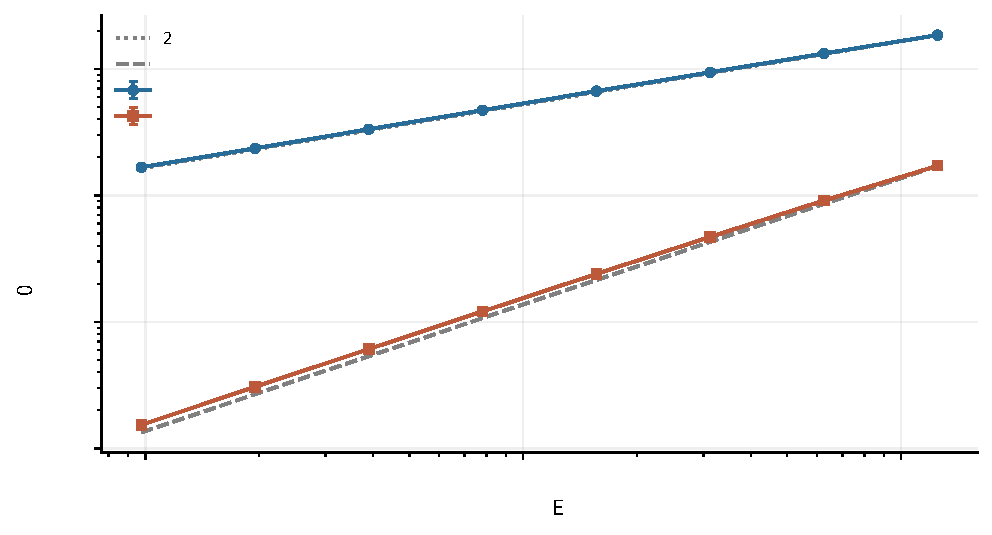
\includegraphics[width=0.88\textwidth,height=0.72\textheight,keepaspectratio]{assets/gbm_strong_cn.pdf}

  \vspace{-0.4em}
  \small 拟合斜率：EM $0.500$；Milstein $0.991$。
\end{frame}

\begin{frame}{怎样解释上一张强误差图？}
  \begin{columns}[T]
    \column{0.52\textwidth}
    \begin{tabular}{lcc}
      \toprule
      方法 & $N=64$ & $N=1024$ \\
      \midrule
      EM & $0.66641$ & $0.16658$ \\
      Milstein & $0.02391$ & $0.00153$ \\
      \bottomrule
    \end{tabular}
    \column{0.44\textwidth}
    \begin{itemize}
      \item $N$ 增大 $16$ 倍，即 $h$ 缩小 $16$ 倍；
      \item EM 误差约缩小 $4$ 倍：$16^{1/2}=4$；
      \item Milstein 误差约缩小 $15.6$ 倍，接近 $16^1$。
    \end{itemize}
  \end{columns}
  \vspace{0.5em}
  \begin{block}{结论}
    数据与理论强阶相符：EM 为 $1/2$，Milstein 为 $1$。这也是代码实现正确的主要验证之一。
  \end{block}
\end{frame}

\begin{frame}{Individual Challenge：改进前后应怎样呈现？}
  \begin{columns}[T]
    \column{0.49\textwidth}
      \centering
      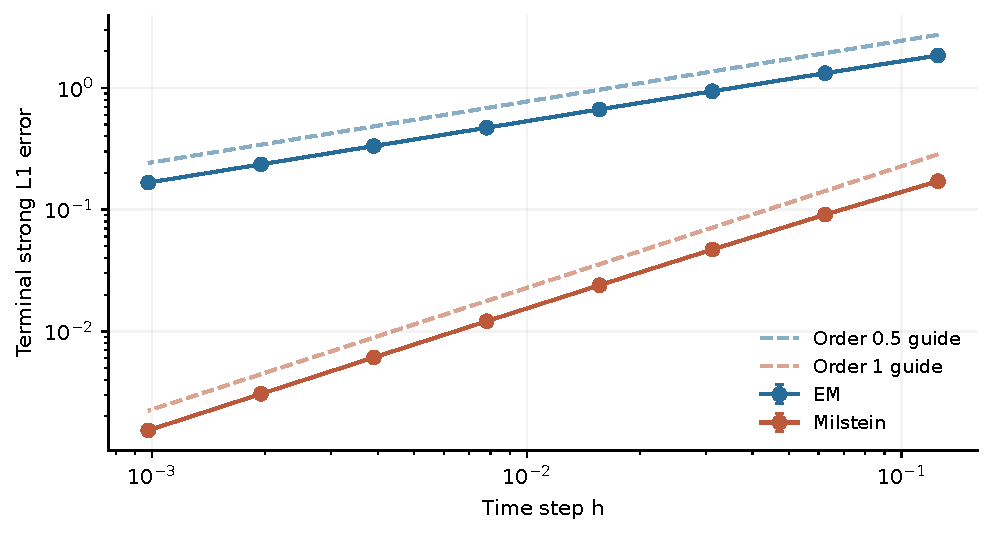
\includegraphics[width=\linewidth,height=0.54\textheight,keepaspectratio]{assets/gbm_strong_before.pdf}

      \small\textbf{改进前：}只有误差曲线，无法判断斜率估计的稳定性。
    \column{0.49\textwidth}
      \centering
      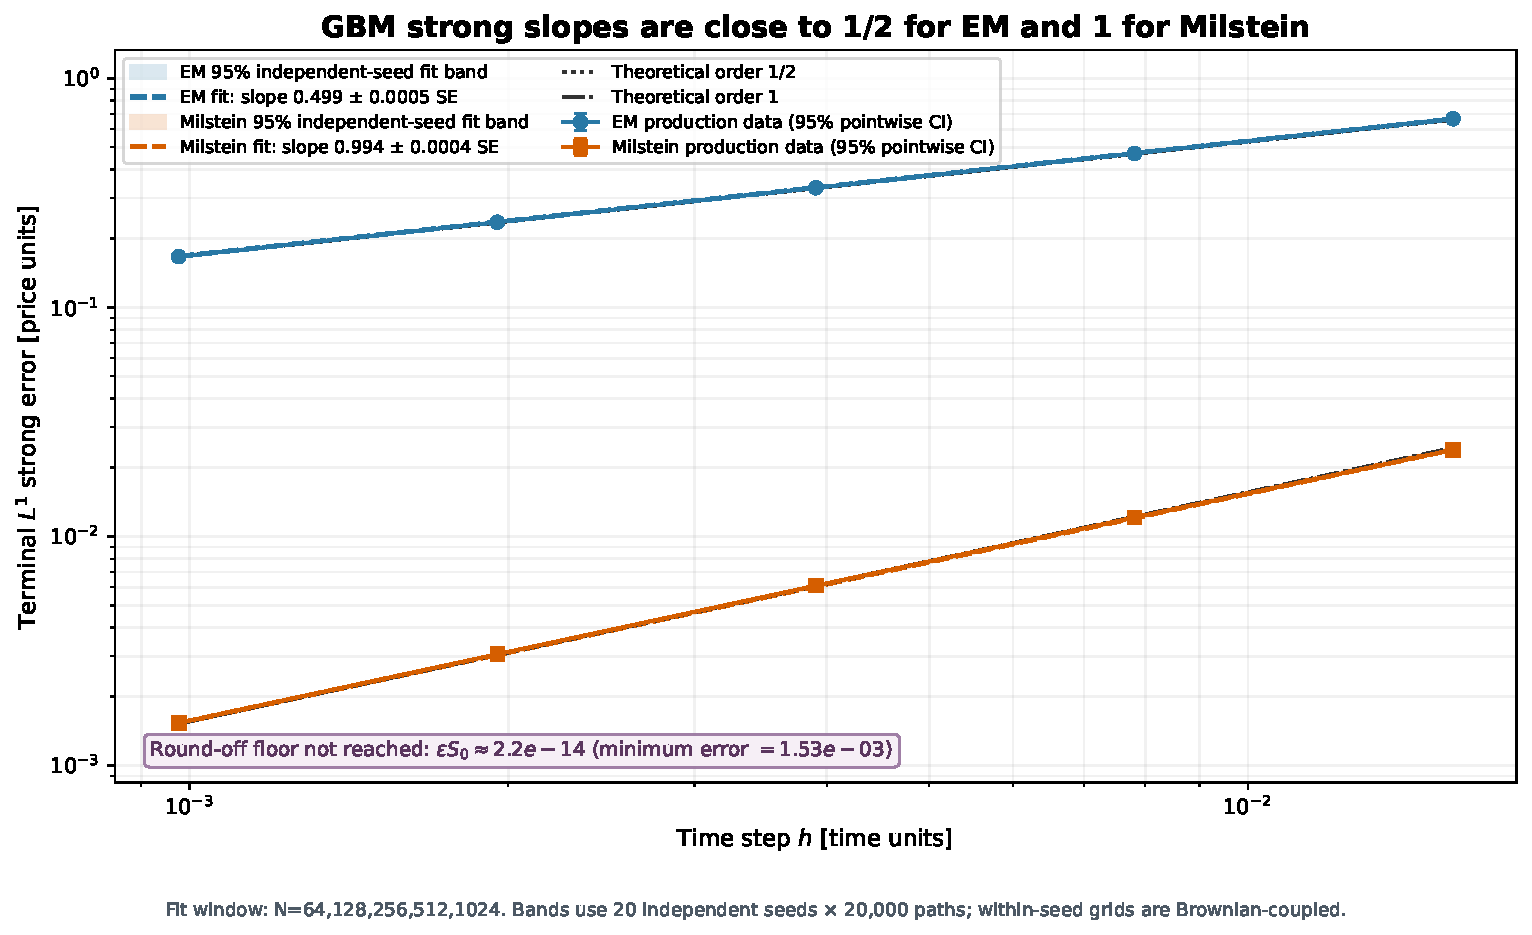
\includegraphics[width=\linewidth,height=0.54\textheight,keepaspectratio]{assets/gbm_strong_improved.pdf}

      \small\textbf{改进后：}增加重复实验误差条、理论参考斜率与拟合斜率。
  \end{columns}
  \vspace{0.2em}
  \centering\footnotesize 把一句“图像看起来符合理论”改成可以量化、检查和复现的证据。
\end{frame}

\begin{frame}{弱误差可以直接解析计算}
  EM 的条件均值满足
  \[
    \E[S_{n+1}^{\rm EM}\mid S_n^{\rm EM}]
      =S_n^{\rm EM}(1+\mu h).
  \]
  递推后
  \[
    \E[S_N^{\rm EM}]=S_0(1+\mu h)^N,
    \qquad N=T/h.
  \]
  Milstein 修正项均值为零，因此其均值与 EM 完全相同：
  \[
    \E[(\Delta W)^2-h]=0.
  \]
  对比真均值 $S_0e^{\mu T}$，得到无 Monte Carlo 噪声的弱误差
  \[
    \boxed{e_{\rm weak}(h)=
      \left|S_0(1+\mu h)^{T/h}-S_0e^{\mu T}\right|=O(h)}.
  \]
\end{frame}

\begin{frame}{GBM 弱收敛结果：为什么两条线重合？}
  \centering
  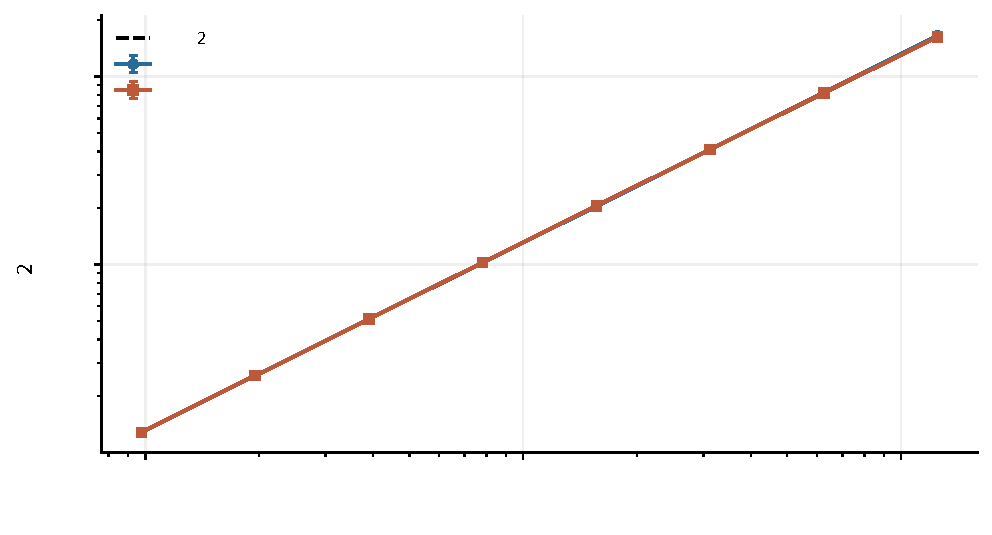
\includegraphics[width=0.88\textwidth,height=0.70\textheight,keepaspectratio]{assets/gbm_weak_cn.pdf}

  \vspace{-0.5em}
  \small EM 拟合斜率 $0.999$，Milstein 拟合斜率 $1.000$；二者对均值这一观测量具有同一个解析偏差。
\end{frame}

\begin{frame}{Milstein 路径更准，为什么均值阶没有提高？}
  \begin{itemize}
    \item Milstein 的额外项改善了每条路径与真路径的匹配，因此强阶提高；
    \item 但该额外项期望为零，没有改变一步条件均值；
    \item 所以对 $\varphi(S)=S$，EM 与 Milstein 的弱误差相同；
    \item 换成其他非线性 $\varphi$ 时，结论可能不同。
  \end{itemize}
  \begin{alertblock}{方法的“阶”必须带上指标}
    ``Milstein 比 EM 高阶''在本项目中准确地说是：对这个一维模型，Milstein 的\emph{强阶}更高；不能据此断言每个弱观测量都更高阶。
  \end{alertblock}
\end{frame}

\begin{frame}{分布检查：误差阶之外的第二道防线}
  \centering
  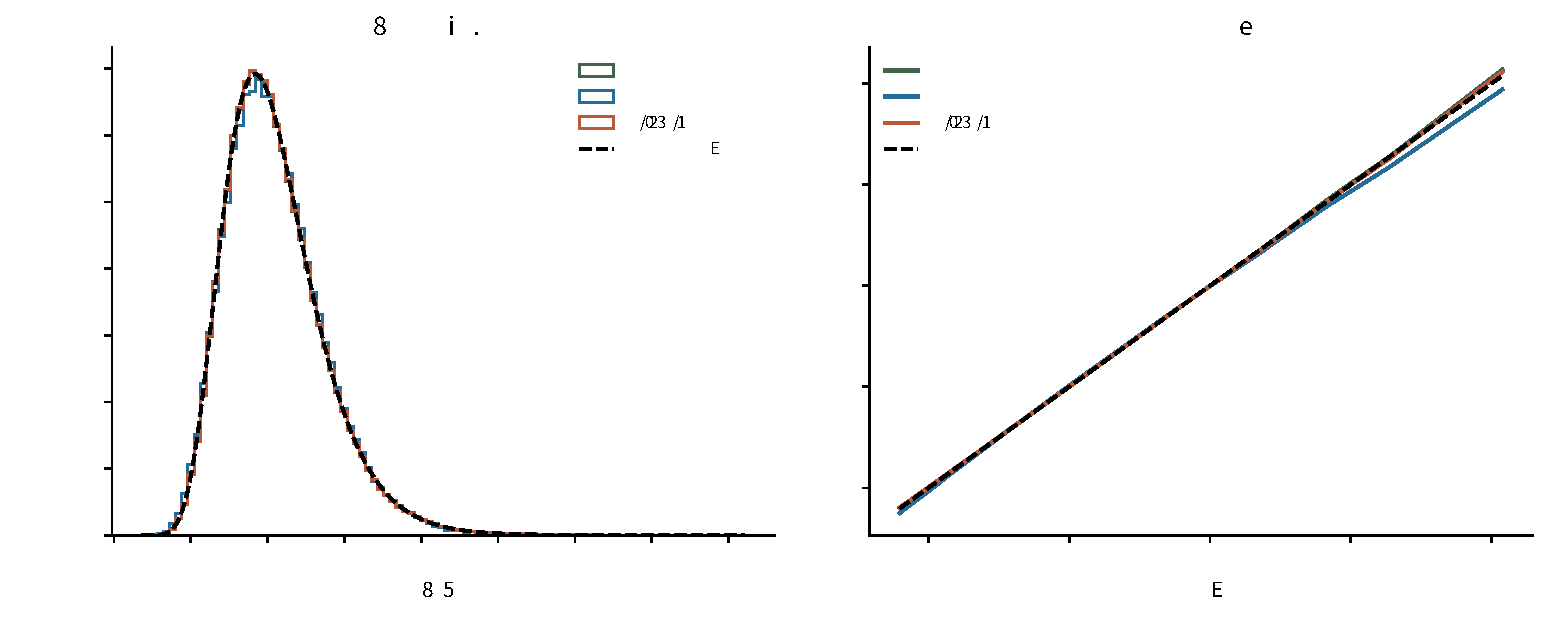
\includegraphics[width=0.88\textwidth,height=0.70\textheight,keepaspectratio]{assets/gbm_distribution_cn.pdf}

  \vspace{-0.5em}
  \small 直方图应与解析对数正态密度一致；经验均值、方差还应落在合理抽样误差内。
\end{frame}

\begin{frame}{正值性检查：明确报告负值频率}
  真解由指数构成，所以 $S_t>0$。离散格式未必自动保持这一性质。
  \begin{center}
    \begin{tabular}{lcc}
      \toprule
      终值生成方式 & 负终值数 / 总路径数 & 经验频率 \\
      \midrule
      精确更新 & $0/160000$ & $0.000\%$ \\
      Euler--Maruyama & $0/160000$ & $0.000\%$ \\
      Milstein & $0/160000$ & $0.000\%$ \\
      \bottomrule
    \end{tabular}
  \end{center}
  \begin{alertblock}{该结果的边界}
    这是本次参数和网格下的\emph{经验终值频率}，不能证明 EM 对所有步长或所有参数都保持正值。
  \end{alertblock}
\end{frame}

\begin{frame}{GBM 阶段得到了什么？}
  \begin{enumerate}
    \item 验证了布朗增量使用 $\sqrt h$ 缩放，并正确复用了同一路径；
    \item 复现 EM 强阶约 $1/2$、Milstein 强阶约 $1$；
    \item 解析解释了二者对终值均值都有一阶弱误差；
    \item 用解析矩、分布图与正值频率补充检查；
    \item 学会了把 log--log 斜率与具体误差缩减倍数对应起来。
  \end{enumerate}
  \begin{block}{下一步}
    去掉解析解这根“拐杖”，在非仿射模型中用更细数值网格充当参考答案。
  \end{block}
\end{frame}

\section{模型二：无解析解时的嵌套网格验证}

\begin{frame}{非仿射模型：状态依赖的随机波动}
  令 $S_t=e^{X_t}$，模型为
  \begin{align*}
    \dd X_t&=\left(\mu-\frac12g(Y_t)^2\right)\dd t+g(Y_t)\dd W_t^{(1)},\\
    \dd Y_t&=\kappa(\theta-Y_t)\dd t
      +\xi\sqrt{1+Y_t^2}\dd W_t^{(2)},\\
    g(y)&=0.1+\frac{0.4}{1+e^{-y}},
    \qquad \operatorname{Corr}(\dd W^{(1)},\dd W^{(2)})=\rho.
  \end{align*}
  \begin{itemize}
    \item $Y_t$ 是辅助状态；$g(Y_t)$ 决定 $X_t$ 的瞬时噪声强度；
    \item $g$ 和 $\sqrt{1+Y^2}$ 都不是仿射函数，因此称为非仿射；
    \item 没有可直接使用的终值解析解。
  \end{itemize}
\end{frame}

\begin{frame}{只需掌握这些参数含义}
  \begin{center}
    \begin{tabular}{clc}
      \toprule
      参数 & 数值分析中的作用 & 本项目值 \\
      \midrule
      $S_0,Y_0$ & 初始条件 & $100,0$ \\
      $\mu$ & $X$ 的平均增长部分 & $0.05$ \\
      $\kappa,\theta$ & $Y$ 拉回中心的速度与中心 & $2,-0.2$ \\
      $\xi$ & $Y$ 的噪声尺度 & $0.6$ \\
      $\rho$ & 两个随机驱动的相关系数 & $-0.7$ \\
      $T$ & 终止时间 & $1$ \\
      \bottomrule
    \end{tabular}
  \end{center}
  \begin{block}{对金融背景的最低要求}
    只需把 $S$ 当作需要模拟的正状态变量，把 $Y$ 当作会改变噪声强度的第二个状态变量。
  \end{block}
\end{frame}

\begin{frame}{怎样生成相关的两个布朗增量？}
  先生成独立标准正态变量 $Z_1,Z_2$，再令
  \[
    \Delta W_1=\sqrt h Z_1,
    \qquad
    \Delta W_2=\sqrt h\left(\rho Z_1+\sqrt{1-\rho^2}Z_2\right).
  \]
  则
  \[
    \Var(\Delta W_1)=\Var(\Delta W_2)=h,
    \qquad
    \operatorname{Corr}(\Delta W_1,\Delta W_2)=\rho.
  \]
  \begin{alertblock}{必须做的数值诊断}
    程序生成后直接计算样本方差和样本相关系数；本实验得到相关系数 $-0.699675$，与目标 $-0.7$ 一致。
  \end{alertblock}
\end{frame}

\begin{frame}{为什么在 $X=\log S$ 上离散？}
  直接更新 $S$ 可能因一个大的负随机增量得到负数。改为更新 $X$ 后再指数变换：
  \[
    S_n=e^{X_n}>0
  \]
  在计算机产生有限浮点数的前提下自动为正。
  \begin{block}{这不是额外金融技巧}
    它是变量变换后的数值格式选择：用解析结构保证状态约束，类似 PDE 中通过变量或通量形式改善离散性质。
  \end{block}
\end{frame}

\begin{frame}{非仿射模型的同步 EM 更新}
  用旧值 $Y_n$ 同时更新两个分量：
  \begin{align*}
    X_{n+1}&=X_n+\left(\mu-\frac12g(Y_n)^2\right)h
      +g(Y_n)\Delta W_{1,n},\\
    Y_{n+1}&=Y_n+\kappa(\theta-Y_n)h
      +\xi\sqrt{1+Y_n^2}\Delta W_{2,n},\\
    S_{n+1}&=e^{X_{n+1}}.
  \end{align*}
  \begin{alertblock}{同步的含义}
    $X_{n+1}$ 和 $Y_{n+1}$ 都只能使用同一个旧状态 $Y_n$。若先覆盖 $Y_n$ 再更新 $X$，实际实现的就不是上述格式。
  \end{alertblock}
\end{frame}

\begin{frame}[fragile]{实现细节：保存旧状态并稳定计算 sigmoid}
\begin{lstlisting}
def g(y):
    # stable sigmoid to avoid exp overflow
    return 0.1 + 0.4 * expit(y)

for n in range(N):
    y_old = y.copy()
    gy = g(y_old)
    x += (mu - 0.5*gy**2)*h + gy*dW1[:, n]
    y += kappa*(theta - y_old)*h \
         + xi*np.sqrt(1.0 + y_old**2)*dW2[:, n]

assert np.isfinite(x).all() and np.isfinite(y).all()
s = np.exp(x)
\end{lstlisting}
  \vspace{-0.4em}
  \small 除了最终图，还应记录：是否出现 NaN/Inf、相关系数、增量方差和负价格数。
\end{frame}

\begin{frame}{一个重要结构：离散均值恰好正确}
  给定 $\mathcal F_n$ 后，$g(Y_n)$ 是已知量。由正态变量的指数矩
  \[
    \E[e^{a\Delta W}]=e^{a^2h/2},
  \]
  有
  \begin{align*}
    \E[S_{n+1}\mid\mathcal F_n]
      &=S_ne^{(\mu-\frac12g_n^2)h}
        \E[e^{g_n\Delta W_{1,n}}]\
      &=S_ne^{\mu h}.
  \end{align*}
  所以
  \[
    \boxed{\E[S_N]=S_0e^{\mu T}\quad\text{对任意步长 }h\text{ 都成立}.}
  \]
  \begin{alertblock}{后果}
    用 $\varphi(S)=S$ 测弱误差会得到理论零偏差，无法检验格式是否正确逼近终值分布。
  \end{alertblock}
\end{frame}

\begin{frame}{为什么选择 call payoff 作为非平凡弱观测量？}
  选取
  \[
    \varphi(S)=(S-K)^+=\max(S-K,0),\qquad K=100.
  \]
  \begin{itemize}
    \item 它是非线性函数，$\E[\varphi(S)]$ 不能只由 $\E[S]$ 决定；
    \item 即使两个离散解均值相同，只要分布的形状或尾部不同，payoff 期望就会不同；
    \item 在 $S=K$ 处有折点，不是光滑测试函数，因此有限样本下弱收敛更难测；
    \item 这里使用它的原因是\alert{数值辨别力}，理解这一点不需要金融定价知识。
  \end{itemize}
  \begin{block}{核心逻辑}
    线性均值被格式结构“自动答对”后，必须换一个会感知分布差异的观测量。
  \end{block}
\end{frame}

\begin{frame}{没有解析解时：用嵌套细网格作参考}
  在同一组最细布朗增量上同时构造：
  \[
    S_T^{N}\quad\text{和}\quad S_T^{N_{\rm ref}},
    \qquad N_{\rm ref}\gg N.
  \]
  粗增量由细增量求和，定义强差
  \[
    \widehat D_N=\frac1M\sum_{i=1}^M
      \left|S_{T,i}^{N}-S_{T,i}^{N_{\rm ref}}\right|.
  \]
  对弱观测量使用配对差
  \[
    \widehat B_N=\frac1M\sum_{i=1}^M
      \left[\varphi(S_{T,i}^{N})-\varphi(S_{T,i}^{N_{\rm ref}})\right].
  \]
  \begin{alertblock}{准确措辞}
    它们是相对于数值参考解的差，不是已知真误差；所以必须做参考网格敏感性检查。
  \end{alertblock}
\end{frame}

\begin{frame}{嵌套实验参数}
  \begin{center}
    \begin{tabular}{ll}
      \toprule
      项目 & 设置 \\
      \midrule
      粗网格 & $N=8,16,32,64,128,256$ \\
      主要参考网格 & $N_{\rm ref}=8192$ \\
      敏感性参考网格 & $2048,4096,8192$ \\
      路径数 & $M=100000$ \\
      随机耦合 & 所有网格聚合同一最细增量 \\
      强量 & $\E|S_T^N-S_T^{N_{\rm ref}}|$ \\
      弱量 & 均值差与 call payoff 配对差 \\
      \bottomrule
    \end{tabular}
  \end{center}
  拟合强阶时只用 $N=8,16,32,64$，避免最细粗网格过度接近有限参考网格而弯曲。
\end{frame}

\begin{frame}{非仿射模型：强差结果}
  \centering
  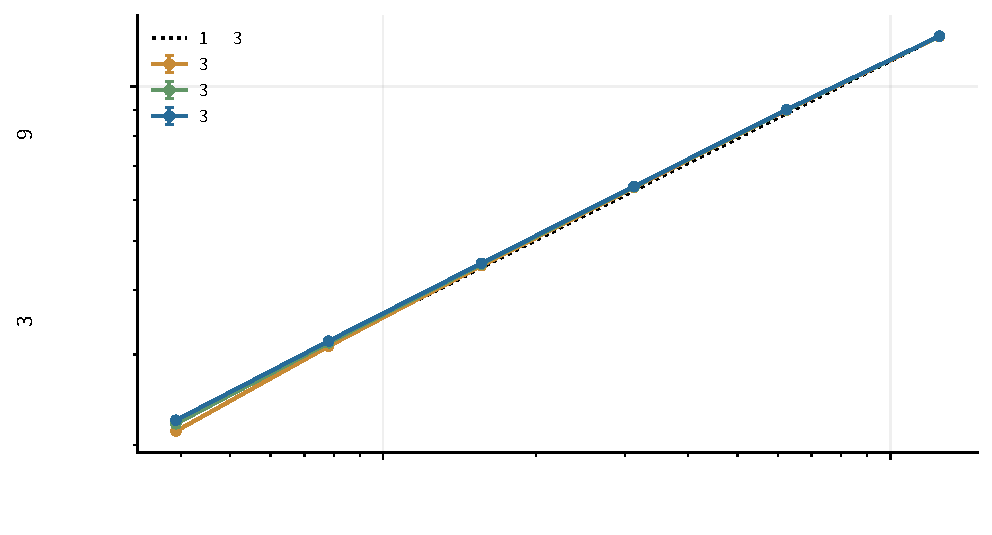
\includegraphics[width=0.88\textwidth,height=0.71\textheight,keepaspectratio]{assets/nonaffine_strong_cn.pdf}

  \vspace{-0.5em}
  \small 相对 $N_{\rm ref}=8192$ 的拟合斜率为 $0.491$，与 EM 的典型强阶 $1/2$ 相容。
\end{frame}

\begin{frame}{怎样证明这个斜率不是参考网格偶然造成？}
  固定拟合粗网格 $N=8,16,32,64$，改变参考网格：
  \begin{center}
    \begin{tabular}{ccc}
      \toprule
      $N_{\rm ref}$ & 拟合斜率 & 对最粗层的解释 \\
      \midrule
      $2048$ & $0.496$ & 参考误差较大，但斜率稳定 \\
      $4096$ & $0.493$ & 与更细参考接近 \\
      $8192$ & $0.491$ & 主报告采用 \\
      \bottomrule
    \end{tabular}
  \end{center}
  \begin{block}{可支持的结论}
    三个参考层给出一致的约 $1/2$ 斜率，因此有较稳健的数值证据支持 EM 型强收敛行为。
  \end{block}
\end{frame}

\begin{frame}{参考解自身误差怎样显现？}
  比较相邻参考层的终值差：
  \[
    \E|S_T^{2048}-S_T^{4096}|\approx0.05679,
    \qquad
    \E|S_T^{4096}-S_T^{8192}|\approx0.04016.
  \]
  比值为
  \[
    \frac{0.04016}{0.05679}\approx0.707\approx2^{-1/2}.
  \]
  \begin{itemize}
    \item 参考层本身也呈现半阶缩减；
    \item 这说明 $8192$ 仍不是“真解”；
    \item 但对较粗的 $N=8$ 到 $64$，它足够细，可观察到稳定渐近斜率。
  \end{itemize}
\end{frame}

\begin{frame}{非仿射模型：弱差与置信区间}
  \centering
  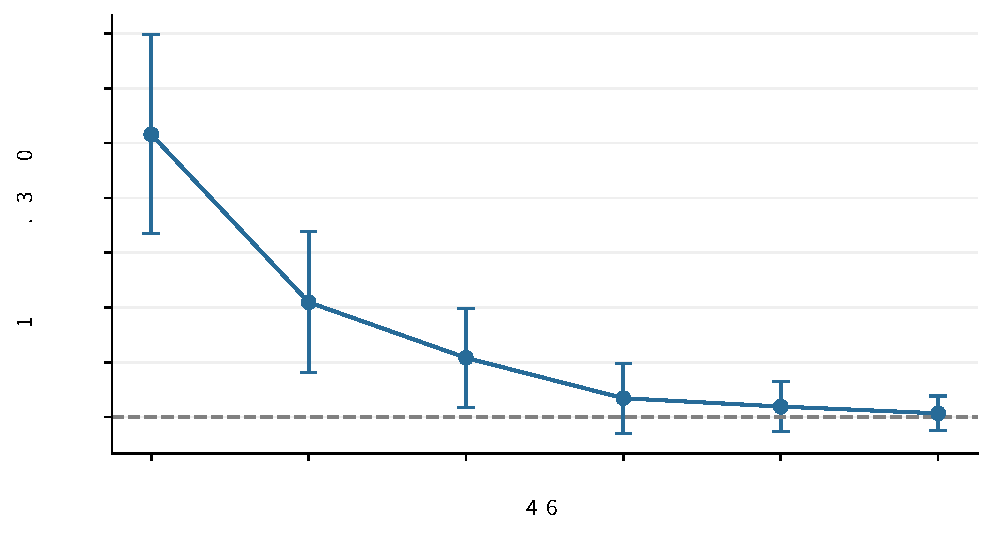
\includegraphics[width=0.88\textwidth,height=0.71\textheight,keepaspectratio]{assets/nonaffine_weak_cn.pdf}

  \vspace{-0.5em}
  \small 粗层 payoff 差可辨认；细层误差条跨过零，Monte Carlo 噪声已与离散差同量级。
\end{frame}

\begin{frame}{为什么这里不能报告可靠弱阶？}
  \begin{itemize}
    \item $N=8,16,32$ 时，payoff 配对差的置信区间不含零；
    \item $N=64,128,256$ 时，置信区间包含零；
    \item 最细层上，误差符号和大小受抽样噪声明显影响；
    \item 对这些点做 log--log 回归会把噪声当成收敛规律；
    \item payoff 有折点，弱误差常数和渐近区间也可能更难辨认。
  \end{itemize}
  \begin{alertblock}{正确结论}
    本实验显示弱偏差随网格细化而减小，但在现有样本预算下\alert{不足以估计可信的弱收敛阶}。这是诚实的数值结论，不是格式被证明失败。
  \end{alertblock}
\end{frame}

\begin{frame}{样本量实验：增加 $M$ 是否解决问题？}
  固定 $N=64$、$N_{\rm ref}=8192$，只改变路径数：
  \begin{center}
    \begin{tabular}{rrrr}
      \toprule
      $M$ & payoff 配对差 & 标准误 & $95\%$ 置信区间 \\
      \midrule
      $10{,}000$  & $0.009045$ & $0.005149$ & $[-0.001048,\ 0.019137]$ \\
      $40{,}000$  & $0.004942$ & $0.002592$ & $[-0.000139,\ 0.010022]$ \\
      $100{,}000$ & $0.001722$ & $0.001633$ & $[-0.001479,\ 0.004923]$ \\
      \bottomrule
    \end{tabular}
  \end{center}
  \begin{itemize}
    \item 标准误大体按 $M^{-1/2}$ 缩小；
    \item 三个区间仍都跨过零；
    \item 说明该层的真实偏差很小，需要更大预算或方差缩减才适合估阶。
  \end{itemize}
\end{frame}

\begin{frame}{均值诊断：精确结构也能检查代码}
  理论上对任意步长
  \[
    \E[S_T^N]=100e^{0.05}=105.1271.
  \]
  最细模拟得到
  \[
    \widehat\E[S_T]=105.08796,
    \qquad 95\%\text{ CI }[104.89962,105.27629].
  \]
  理论值落在区间内。对应 payoff 估计为
  \[
    14.53804,
    \qquad 95\%\text{ CI }[14.40515,14.67093].
  \]
  \begin{block}{两种角色}
    均值用于检查实现；payoff 用于观察非平凡分布偏差。不要强迫同一个统计量承担两项任务。
  \end{block}
\end{frame}

\begin{frame}{数值诊断清单}
  \begin{center}
    \begin{tabularx}{\textwidth}{>{\bfseries}p{3.5cm}X}
      \toprule
      检查项 & 本项目观察 \\
      \midrule
      布朗增量方差 & 与目标最细步长 $1/8192\approx1.221\times10^{-4}$ 一致 \\
      两驱动相关系数 & $-0.699675$，目标为 $-0.7$ \\
      有限性 & 所有报告路径的 $X,Y,S$ 均为有限数 \\
      正值性 & $S=e^X$，模拟价格保持正值 \\
      精确均值结构 & 理论值落在经验 $95\%$ 区间内 \\
      参考层敏感性 & 三个参考网格给出相近强斜率 \\
      \bottomrule
    \end{tabularx}
  \end{center}
  一张漂亮的收敛图不能替代这些基本检查。
\end{frame}

\section{如何评价结果与组织代码}

\begin{frame}{哪些结论是任务真正要求的？}
  \begin{tabularx}{\textwidth}{>{\bfseries}p{3.3cm}XX}
    \toprule
    内容 & 应做 & 本项目证据 \\
    \midrule
    GBM 强收敛 & 比较 EM、Milstein 理论阶 & $0.500$ 与 $0.991$ \\
    GBM 弱行为 & 选定观测量并解释 & 均值偏差解析一阶 \\
    分布/正值检查 & 定量报告 & 矩、直方图、负值频率 \\
    非仿射强验证 & 嵌套网格与敏感性 & 稳定约半阶 \\
    非仿射弱验证 & 置信区间与谨慎结论 & 趋势可见，阶不可可靠估计 \\
    复现性 & 命令、种子、环境、Git & 代码与输出可追溯 \\
    \bottomrule
  \end{tabularx}
  \vspace{0.6em}
  ``测出的弱阶''不是必须成功等于某个漂亮数字；必须做的是采用合理实验并报告证据的限度。
\end{frame}

\begin{frame}{代码结构应当对应数学结构}
  \begin{enumerate}
    \item \textbf{参数层}：初值、系数、$T$、网格、路径数、随机种子；
    \item \textbf{随机增量层}：生成最细独立正态数，构造相关增量；
    \item \textbf{求解器层}：EM、Milstein、对数 EM；
    \item \textbf{耦合层}：细增量求和得到各个粗网格输入；
    \item \textbf{统计层}：误差均值、标准误、置信区间、回归斜率；
    \item \textbf{输出层}：表格、图、机器可读数据和运行元数据。
  \end{enumerate}
  \begin{block}{好处}
    若图中某个点异常，可以沿着“数据—统计量—路径—随机增量—参数”逐层定位，而不是在一个大脚本里猜测。
  \end{block}
\end{frame}

\begin{frame}{复现一个报告数字的最小闭环}
  \centering
  \begin{tikzpicture}[
    node distance=6mm,
    box/.style={draw=CourseNavy,rounded corners,fill=CourseLight,
      minimum width=6.7cm,minimum height=7mm,align=center,font=\small},
    arr/.style={-{Latex[length=2mm]},thick,draw=CourseTeal}
  ]
    \node[box] (c) {锁定 Git commit：代码、参数与文档版本};
    \node[box,below=of c] (cmd) {使用报告记录的完整命令行};
    \node[box,below=of cmd] (env) {固定随机种子并记录 Python / NumPy 版本};
    \node[box,below=of env] (out) {保存原始输出与图表数据};
    \node[box,below=of out] (match) {核对报告数字到指定有效位数};
    \draw[arr] (c)--(cmd);
    \draw[arr] (cmd)--(env);
    \draw[arr] (env)--(out);
    \draw[arr] (out)--(match);
  \end{tikzpicture}
  \vspace{0.6em}

  如果脚本输出与报告不一致，应修正报告或查清版本，而不是只保留更好看的数字。
\end{frame}

\begin{frame}{最容易犯的八个错误}
  \begin{enumerate}
    \item 把 $\Delta W$ 写成 $hZ$，遗漏 $\sqrt h$；
    \item 强误差比较时使用独立随机路径；
    \item 把样本方差当作估计均值的标准误；
    \item 只减小 $h$，却不检查 Monte Carlo 噪声平台；
    \item 更新 $Y$ 后才用新 $Y$ 更新 $X$，破坏同步 EM 格式；
    \item 把有限细网格称为“精确解”；
    \item 对跨零且符号不稳的弱偏差强行做 log--log 拟合；
    \item 只报告斜率，不报告拟合区间、误差条和诊断。
  \end{enumerate}
\end{frame}

\begin{frame}{如何读一张合格的收敛图？}
  按以下顺序提问：
  \begin{enumerate}
    \item 横轴是 $h$、$N$ 还是计算成本？方向是否反转？
    \item 纵轴具体是什么误差？是真误差、参考差还是绝对偏差？
    \item 粗细解是否共享同一随机输入？
    \item 误差条表示标准差、标准误还是置信区间？
    \item 斜率在哪些点上拟合？为何选择这些点？
    \item 最细点是否进入 Monte Carlo 噪声平台或参考误差平台？
    \item 改变样本量或参考层后，结论是否稳定？
  \end{enumerate}
  \begin{alertblock}{一条实用规则}
    先确认纵轴“测的是什么”，再看线是否直，最后才读拟合斜率。
  \end{alertblock}
\end{frame}

\begin{frame}{项目的主要结论}
  \begin{enumerate}
    \item 在 GBM 基准上，EM 与 Milstein 的强阶分别约为 $1/2$ 和 $1$，与理论一致；
    \item 对终值均值，二者共享同一个一阶弱偏差，说明强阶提高不等于每个弱量都提高；
    \item 在非仿射模型上，嵌套参考实验稳定显示约 $1/2$ 的强收敛行为；
    \item 非仿射离散均值对所有步长都精确，所以非线性 payoff 才能检验分布偏差；
    \item 现有路径数只能支持“弱偏差趋于减小”，不足以给出可信弱阶；
    \item 置信区间、参考层敏感性和运行诊断与拟合斜率同样重要。
  \end{enumerate}
\end{frame}

\begin{frame}{如果继续改进，优先做什么？}
  \begin{enumerate}
    \item 对 payoff 弱误差使用更多配对样本，或加入控制变量降低方差；
    \item 在固定计算预算下平衡 $h$ 与 $M$，避免某一种误差远小于另一种；
    \item 进一步加细参考网格，量化参考解带来的系统偏差；
    \item 报告回归斜率的置信区间，而不只给点估计；
    \item 若课程希望比较 PDE 与 Monte Carlo，可在一维简化模型上增加有限差分解作交叉验证。
  \end{enumerate}
  \begin{block}{本科作业的合理边界}
    这些是后续方向。当前报告最重要的是把已有方法、证据和局限解释清楚，而不是继续堆叠更复杂技术。
  \end{block}
\end{frame}

\begin{frame}[plain]
  \vfill
  \centering
  {\Huge\color{CourseNavy}谢谢！}

  \vspace{1em}
  {\Large Questions?}

  \vspace{2em}
  \begin{minipage}{0.78\textwidth}
    \centering
    \color{CourseTeal}
    从欧拉法出发，我们只增加了三样东西：
    \textbf{正态增量、重复抽样、误差的统计量化}。
  \end{minipage}
  \vfill
\end{frame}

\appendix
\section{备用推导与答疑页}

\begin{frame}{备用：GBM 均值偏差为何是一阶？}
  令 $N=T/h$。使用展开
  \[
    \log(1+\mu h)=\mu h-\frac12\mu^2h^2+O(h^3),
  \]
  则
  \begin{align*}
    (1+\mu h)^{T/h}
      &=\exp\!\left[\frac{T}{h}\log(1+\mu h)\right]\\
      &=\exp\!\left[\mu T-\frac12\mu^2Th+O(h^2)\right]\\
      &=e^{\mu T}\left(1-\frac12\mu^2Th+O(h^2)\right).
  \end{align*}
  因而
  \[
    S_0(1+\mu h)^{T/h}-S_0e^{\mu T}=O(h).
  \]
\end{frame}

\begin{frame}{备用：为什么配对差能降低弱误差噪声？}
  两种估计方式：
  \begin{align*}
    \text{独立：}\quad
      &\widehat\E[\varphi(S^N)]-\widehat\E[\varphi(S^{\rm ref})],\\
    \text{配对：}\quad
      &\frac1M\sum_i\left[
        \varphi(S_i^N)-\varphi(S_i^{\rm ref})\right].
  \end{align*}
  对配对差，单个样本的方差是
  \[
    \Var(A-B)=\Var(A)+\Var(B)-2\Cov(A,B).
  \]
  共享布朗路径使 $A,B$ 高度正相关，协方差项显著降低差值方差。
  \begin{block}{直观理解}
    同一次随机冲击把粗、细解一起推高或推低；相减时共同波动抵消，剩下的主要是离散差。
  \end{block}
\end{frame}

\begin{frame}{备用：标准误与样本量}
  若配对差样本为 $D_1,\ldots,D_M$，则
  \[
    \bar D=\frac1M\sum_iD_i,
    \qquad
    s_D^2=\frac1{M-1}\sum_i(D_i-\bar D)^2,
    \qquad
    \operatorname{SE}(\bar D)=\frac{s_D}{\sqrt M}.
  \]
  若希望标准误从 $\varepsilon_1$ 降到 $\varepsilon_2$，粗略需要
  \[
    M_2\approx M_1\left(\frac{\varepsilon_1}{\varepsilon_2}\right)^2.
  \]
  例如将标准误缩小到原来的 $1/5$，路径数需约增加到 $25$ 倍。
\end{frame}

\begin{frame}{备用：术语速查}
  \begin{tabularx}{\textwidth}{>{\bfseries}p{3.1cm}X}
    \toprule
    术语 & 本项目中的意思 \\
    \midrule
    漂移 drift & 每单位时间的平均确定性变化 \\
    扩散 diffusion & 随机扰动的幅度 \\
    布朗增量 & 均值 $0$、方差 $h$ 的正态随机量 \\
    路径 path & 一整串 $Z_0,Z_1,\ldots,Z_N$ \\
    观测量 observable & 对终值取的函数 $\varphi(Z_T)$ \\
    强收敛 & 同一路径上的数值解接近真解 \\
    弱收敛 & 某个观测量的期望接近真值 \\
    嵌套网格 & 粗增量由同一批细增量求和得到 \\
    数值参考解 & 很细网格解，用于近似未知真解 \\
    \bottomrule
  \end{tabularx}
\end{frame}

\begin{frame}{参考资料与项目文件}
  \begin{thebibliography}{9}
    \bibitem{problem-pack}
    课程 Problem Pack，Direction 4：Financial SDEs，pp.~6--7.

    \bibitem{higham}
    D.~J. Higham,
    \newblock An Algorithmic Introduction to Numerical Simulation of Stochastic Differential Equations,
    \newblock \emph{SIAM Review}, 43(3), 2001.

    \bibitem{kloeden-platen}
    P.~E. Kloeden and E.~Platen,
    \newblock \emph{Numerical Solution of Stochastic Differential Equations},
    \newblock Springer, 1992.
  \end{thebibliography}
  \vspace{0.3em}
  \small 项目脚本：\code{gbm.py}、\code{nonaffine.py}；本科版报告：\code{undergraduate\_revision/}。
\end{frame}

\end{document}
